\RequirePackage{fix-cm}

\documentclass[smallextended,natbib]{svjour3}

\smartqed

\usepackage{graphicx}
\usepackage{amsmath}
\usepackage{amssymb}
\usepackage{booktabs}
\usepackage[section]{placeins}
\usepackage{url}
\setlength{\emergencystretch}{2em}

\journalname{Lifetime Data Analysis}

\begin{document}

\raggedbottom

\title{Grouped Proportional Hazards under Coarse Time: Information Loss and Baseline Estimation}
\titlerunning{Grouped Proportional Hazards under Coarse Time}

\author{Simhaa T. T. \and Sudheesh Kumar Kattumannil}
\authorrunning{Simhaa and Kattumannil}

\institute{Simhaa T. T. \at Department of Electrical and Electronics Engineering, Sri Sivasubramaniya Nadar College of Engineering, Chennai, Tamil Nadu, India\\ Corresponding author: \email{simhaa2310510@ssn.edu.in}\\ ORCID: 0009-0006-9041-1103 \and Sudheesh Kumar Kattumannil \at Applied Statistics Unit, Indian Statistical Institute, Chennai, Tamil Nadu, India\\ \email{skkattu@isichennai.res.in}}

\maketitle

\begin{abstract}
Event times recorded on a coarse grid create two related problems: temporal grouping removes information, and tied failures complicate prediction from a Cox model. We first derive an exact finite-grid identity for Fisher information lost when a continuous survival time is grouped. For an equally spaced refining grid, the loss is quadratic in the interval width. A corresponding expansion is obtained after profiling an interval-specific baseline. We then examine why held-out interval likelihoods from grouped proportional hazards fits can differ from predictions obtained after Cox regression. In 34 configurations from eight public cohorts, Cox coefficients estimated with Efron's tie approximation and combined with a Breslow baseline gave a positive grouped-minus-Cox advantage, expressed as a Cox-minus-grouped negative log-likelihood difference, in 29 configurations. Replacing only the baseline by the Kalbfleisch--Prentice profile estimator reduced the difference to zero or below in 31 configurations; none of the remaining positive differences was resolved by the corrected repeated-split standard error. In four independent SPARCS cohorts, 3 of 12 profile-baseline differences were resolved, but their magnitudes were 1.33\% or less of the corresponding Breslow differences. A controlled simulation further showed that event-tie concentration, rather than concentration of all exit times, orders the predictive discrepancy. The results separate information loss due to grouping from the baseline-estimation effect that dominates the usual Cox prediction comparison under heavy ties.
\keywords{Grouped survival data \and Proportional hazards \and Tied event times \and Baseline survival estimation \and Fisher information \and Discrete-time survival analysis}
\end{abstract}

\section{Introduction}
\label{sec:introduction}

Event times are often observed on a grid. Hospital length of stay is typically recorded in whole days, whereas other survival outcomes may be measured more finely and subsequently grouped for analysis. Both situations produce repeated event times, but they do not have the same statistical interpretation. If a latent continuous failure time exists, the grid is a coarsening device. If time is intrinsically discrete, the categories are part of the observation scale itself \citep{tutz2016,nawata2009}.

For a continuous proportional hazards process, grouping over intervals gives an exact complementary-log-log model with the same covariate coefficient \citep{prentice1978}. This identity is sometimes obscured when tied data are analysed through a Cox partial likelihood. Cox regression estimates the regression coefficient without estimating the baseline hazard directly \citep{cox1972,andersen1993}. Prediction of interval probabilities, however, requires the baseline to be reconstructed after the coefficient has been fitted. The usual choices made at these two stages need not have the same statistical status. Efron's and Breslow's approximations concern tied risk sets in the partial likelihood \citep{breslow1974,efron1977}; the Breslow and Kalbfleisch--Prentice estimators concern the baseline survival used for prediction \citep{kalbfleisch1973,prentice2003,xia2018}.

Grouped likelihood and a standard Cox prediction pipeline can give different held-out interval likelihoods on coarse grids. That difference need not imply a different proportional-hazards link. Conditional on a fixed Cox coefficient, the Kalbfleisch--Prentice baseline is the profile maximum-likelihood baseline for the grouped complementary-log-log model. This gives a direct decomposition in which the coefficient, test observations and time grid are held fixed while only the baseline estimator changes. The algebra behind the profile estimator is classical \citep{kalbfleisch1973,allison1982}; here it is used to identify the source of the predictive discrepancy.

A separate question concerns information lost by grouping. Corrections of quadratic order in the grouping width are classical, beginning with Sheppard-type corrections \citep{sheppard1897}. For Cox regression, grouping effects were studied by \citet{mckeague1994,mckeague1996}, and \citet{felsenstein1998} considered asymptotic information loss under a different information criterion. We derive an exact finite-grid identity for a local proportional-hazards direction. The identity gives strict positivity of the loss and yields a quadratic small-bin expansion with an explicit survival-dependent coefficient. We also profile an interval-specific baseline and obtain the corresponding leading term.

The paper has three aims. First, it separates the observation-scale question from the estimation question by distinguishing a refining grid from a fixed discrete grid. Second, it gives finite-grid and small-bin expressions for the information cost of grouping. Third, it decomposes the predictive difference between grouped joint maximum likelihood and Cox-based interval prediction into a coefficient component and a baseline-estimation component. The empirical analysis uses 20 repeated train--test splits with a corrected repeated-split standard error \citep{nadeau2003}. A controlled simulation is used to determine whether the relevant concentration statistic is the modal mass of all exits or the modal mass of failures. A secondary analysis of flexible covariate effects is reported in the Supplementary Material; it is not needed for the main argument.

\section{Observation scale and grouped proportional hazards}
\label{sec:model}

\subsection{Observation scheme}
\label{sec:observation}

Let $T^\ast\in(0,\infty)$ denote a failure time, $C$ a censoring time, and $X\in\mathcal X\subset\mathbb R^d$ a vector of covariates. When a latent continuous failure time is meaningful, write
\begin{equation}
\Lambda(s\mid x)=\int_0^s\lambda(v\mid x)\,dv,
\qquad
S(s\mid x)=\exp\{-\Lambda(s\mid x)\},
\label{eq:survival}
\end{equation}
where $\lambda$ is the conditional hazard. Fix a finite horizon $\tau$ and a grid
\begin{equation}
0=a_0<a_1<\cdots<a_T=\tau,
\qquad I_t=(a_{t-1},a_t].
\label{eq:grid}
\end{equation}
For a continuous hazard, define the integrated hazard in interval $I_t$ by
\begin{equation}
u_t(x)=\int_{I_t}\lambda(s\mid x)\,ds.
\label{eq:integrated-hazard}
\end{equation}

The observed record for subject $i$ is $(E_i,K_i,\delta_i,X_i)$, where $E_i$ is the first interval in which the subject is at risk, $K_i$ is the exit interval, and $\delta_i$ indicates failure at exit. The corresponding interval hazard is
\begin{equation}
h_t(x)=\Pr\{T^\ast\in I_t\mid T^\ast>a_{t-1},X=x\}.
\label{eq:interval-hazard}
\end{equation}
For intrinsically discrete time, Eq.~\eqref{eq:interval-hazard} is defined directly and no latent continuous $T^\ast$ is required \citep{tutz2016}.

Two regimes are useful. In regime R1, a continuous or sufficiently fine event time is available before the analyst imposes a grid. Refining the grid is meaningful, and $\Delta\to0$ can be used to study information loss. In regime R2, the categories are the recorded time scale. The number and meaning of those categories are features of the data rather than asymptotic approximations to an unobserved ordering. The labels R1 and R2 describe the observation scheme used in an analysis; they do not assert a biological property of a dataset.

\subsection{Exact grouped representation}
\label{sec:grouped-representation}

For grouped continuous time,
\begin{equation}
h_t(x)=1-\frac{S(a_t\mid x)}{S(a_{t-1}\mid x)}
       =1-\exp\{-u_t(x)\}.
\label{eq:grouped-hazard}
\end{equation}
Under proportional hazards,
\begin{equation}
\lambda(s\mid x)=\lambda_0(s)\exp\{g(x)\},
\label{eq:ph}
\end{equation}
so
\begin{equation}
u_t(x)=\exp\{g(x)\}\int_{I_t}\lambda_0(s)\,ds.
\end{equation}
With
\begin{equation}
\alpha_t=\log\int_{I_t}\lambda_0(s)\,ds,
\end{equation}
Eq.~\eqref{eq:grouped-hazard} becomes
\begin{equation}
\log\{-\log[1-h_t(x)]\}=\alpha_t+g(x),
\qquad
h_t(x)=1-\exp[-\exp\{\alpha_t+g(x)\}].
\label{eq:cloglog}
\end{equation}
Thus grouping a continuous proportional hazards model does not change the covariate effect; it changes the interval baseline \citep{prentice1978}. The same equation can also be specified directly on a discrete time scale \citep{allison1982,tutz2016}.

Let
\begin{equation}
y_{it}=\delta_i\mathbf 1\{K_i=t\}.
\end{equation}
If entry and censoring occur on interval boundaries and censoring is conditionally independent given $X$, the grouped likelihood is
\begin{equation}
L(\alpha,g)=
\prod_{i=1}^n\prod_{t=E_i}^{K_i}
 h_t(X_i)^{y_{it}}\{1-h_t(X_i)\}^{1-y_{it}}.
\label{eq:grouped-likelihood}
\end{equation}
This is the standard person-period Bernoulli representation \citep{prentice1978,tutz2016}. If censoring occurs inside an interval, a full-interval contribution is not exact. Section~\ref{sec:sensitivity} reports a partial-interval sensitivity analysis for that case.

\subsection{Cox coefficients and baseline reconstruction}
\label{sec:cox-baselines}

For $g(x)=\beta^\top x$, Cox regression estimates $\beta$ from the partial likelihood \citep{cox1972}. When $d_j$ failures occur at the same recorded time $\tau_j$, Efron's approximation is
\begin{equation}
L_{E,j}(\beta)=
\frac{\exp\{\beta^\top\sum_{i\in D_j}X_i\}}
{\displaystyle\prod_{\ell=0}^{d_j-1}
\left[\sum_{k\in R_j}e^{\beta^\top X_k}
-\frac{\ell}{d_j}\sum_{i\in D_j}e^{\beta^\top X_i}\right]},
\label{eq:efron}
\end{equation}
where $D_j$ is the tied failure set and $R_j$ is the risk set \citep{efron1977}. The empirical analyses use the Efron coefficient estimate $\widehat\beta_E$ unless stated otherwise.

A coefficient estimate alone does not determine interval probabilities. A baseline estimate is also required. Write
\begin{equation}
r_i=\exp(\widehat\beta_E^\top X_i).
\end{equation}
For a grid interval with $d_t$ failures and risk set $R_t$, the Breslow cumulative-baseline increment is
\begin{equation}
\Delta\widehat\Lambda_{0,B,t}
 =\frac{d_t}{\sum_{i\in R_t}r_i}.
\label{eq:breslow-baseline}
\end{equation}
The resulting interval failure probability is
\begin{equation}
\widehat h_{B,t}(x)=
1-\exp\{-\Delta\widehat\Lambda_{0,B,t}\exp(\widehat\beta_E^\top x)\}.
\label{eq:breslow-prediction}
\end{equation}
The Breslow estimator is widely used after Cox regression \citep{breslow1974,xia2018}.

A different baseline follows by profiling the grouped likelihood while holding $\beta$ fixed. Put $a_t=\exp\{-\exp(\alpha_t)\}$, the baseline conditional survival across interval $t$. The profile score equation is
\begin{equation}
\sum_{i\in D_t}\frac{r_i}{1-a_t^{r_i}}
=
\sum_{i\in R_t}r_i.
\label{eq:kp-score}
\end{equation}
Its solution gives
\begin{equation}
\widehat h_{KP,t}(x)=1-\widehat a_t^{\exp(\widehat\beta_E^\top x)}.
\label{eq:kp-prediction}
\end{equation}
This is the Kalbfleisch--Prentice baseline construction and, conditional on $\beta$, the profile maximum-likelihood baseline for the grouped complementary-log-log model \citep{kalbfleisch1973,allison1982}. The relation is classical. We use it to isolate the contribution of baseline estimation; no novelty is claimed for Eq.~\eqref{eq:kp-score}. Earlier empirical comparisons of Breslow and Kalbfleisch--Prentice survival estimators have also reported differences in bias and mean squared error \citep{xia2018}.

\section{Information lost by grouping}
\label{sec:information}

\subsection{Finite-grid identity}
\label{sec:information-exact}

Consider regime R1, condition on $X=x$, and suppose subjects enter at zero and are administratively censored at $\tau$. For a scalar local parameter that adds to the log integrated hazard, write $u=e^\eta$ and $h=1-e^{-u}$. The Bernoulli Fisher information for $\eta$ is \citep{vanderVaart1998}
\begin{equation}
g(u)=\frac{(\partial h/\partial\eta)^2}{h(1-h)}
    =\frac{u^2e^{-u}}{1-e^{-u}}.
\label{eq:g-info}
\end{equation}
A subject contributes grouped information from interval $I_t$ only after surviving to its left endpoint. Hence
\begin{equation}
\mathcal I_T(x)=\sum_{t=1}^T S(a_{t-1}\mid x)g\{u_t(x)\}.
\label{eq:grouped-info}
\end{equation}
With the continuous failure time observed up to $\tau$,
\begin{equation}
\mathcal I_\infty(x)=\int_0^\tau S(s\mid x)\lambda(s\mid x)\,ds
=1-S(\tau\mid x).
\label{eq:continuous-info}
\end{equation}

\begin{lemma}
\label{lem:exact}
For any finite grid in Eq.~\eqref{eq:grid} with $0<u_t(x)<\infty$,
\begin{equation}
\mathcal I_\infty(x)-\mathcal I_T(x)
=
\sum_{t=1}^T S(a_{t-1}\mid x)\psi\{u_t(x)\},
\label{eq:exact-loss}
\end{equation}
where
\begin{equation}
\psi(u)=(1-e^{-u})-\frac{u^2e^{-u}}{1-e^{-u}}.
\label{eq:psi}
\end{equation}
\end{lemma}

\begin{proof}
For each interval,
\begin{equation}
\int_{I_t}S(s\mid x)\lambda(s\mid x)\,ds
=S(a_{t-1}\mid x)\{1-e^{-u_t(x)}\}.
\end{equation}
Summing over intervals and subtracting Eq.~\eqref{eq:grouped-info} gives Eq.~\eqref{eq:exact-loss}.
\end{proof}

The identity does not require equal interval widths or an asymptotic grid sequence.

\begin{lemma}
\label{lem:positive}
For every $u>0$, $\psi(u)>0$. Therefore $\mathcal I_T(x)<\mathcal I_\infty(x)$ whenever an interval has positive hazard.
\end{lemma}

\begin{proof}
Because $1-e^{-u}>0$,
\begin{align}
\psi(u)>0
&\iff(1-e^{-u})^2>u^2e^{-u}\\
&\iff\{e^{u/2}-e^{-u/2}\}^2>u^2\\
&\iff 2\sinh(u/2)>u.
\end{align}
The last inequality is strict for $u>0$.
\end{proof}

\subsection{Small-bin expansion}
\label{sec:small-bin}

The local expansion is
\begin{equation}
\psi(u)=\frac{u^3}{12}-\frac{u^4}{24}+\frac{7u^5}{720}+O(u^6),
\qquad u\downarrow0.
\label{eq:psi-expansion}
\end{equation}
It follows from the Bernoulli-number expansion of $u/(e^u-1)$.

For the next result, let $a_t=t\Delta$, with $\Delta=\tau/T$. Assume that $\lambda(s\mid x)$ is uniformly bounded on $[0,\tau]\times\mathcal X$ and continuously differentiable in $s$, with the derivative uniformly bounded.

\begin{theorem}
\label{thm:small-bin}
Under these conditions,
\begin{equation}
\mathcal I_\infty(x)-\mathcal I_T(x)
=
\frac{\Delta^2}{12}
\int_0^\tau S(s\mid x)\lambda(s\mid x)^3\,ds
+O(\Delta^3),
\label{eq:small-bin-loss}
\end{equation}
uniformly in $x$.
\end{theorem}

\begin{proof}
Uniform boundedness gives $u_t(x)=O(\Delta)$ uniformly. By Eq.~\eqref{eq:psi-expansion},
$\psi\{u_t(x)\}=u_t(x)^3/12+O(\Delta^4)$. For some $\zeta_t\in I_t$,
$u_t(x)=\Delta\lambda(\zeta_t\mid x)$. Substitution into Eq.~\eqref{eq:exact-loss} gives
\begin{equation}
\mathcal I_\infty(x)-\mathcal I_T(x)
=
\frac{\Delta^3}{12}\sum_{t=1}^T
S(a_{t-1}\mid x)\lambda(\zeta_t\mid x)^3
+O(T\Delta^4).
\end{equation}
Since $T=\tau/\Delta$, the remainder is $O(\Delta^3)$. The first term is a Riemann sum; the stated smoothness gives the same order for its approximation error.
\end{proof}

The $\Delta^2$ order is consistent with the classical family of grouping corrections \citep{sheppard1897,mckeague1994,mckeague1996,felsenstein1998}. Equation~\eqref{eq:small-bin-loss} supplies the coefficient for the present local proportional-hazards direction. It is a statement about R1. It does not prescribe a fictitious continuous scale for an intrinsically discrete outcome.

\subsection{Profiling an interval-specific baseline}
\label{sec:profiled-info}

The preceding calculation treats the interval baseline as known. To quantify the effect of estimating it, consider
\begin{equation}
\eta_t(x)=\alpha_t+\beta v(x),
\end{equation}
where $v$ is a scalar covariate direction and $\alpha=(\alpha_1,\ldots,\alpha_T)^\top$ is unknown. Let
\begin{equation}
\pi_t(x)=\Pr(E\le t\le K\mid X=x),
\qquad
W_t(x)=\pi_t(x)g\{u_t(x)\}.
\end{equation}

\begin{lemma}
\label{lem:profile-info}
The Fisher information for $\beta$ after profiling $\alpha$ is
\begin{equation}
\mathcal I_T^\star
=
\sum_{t=1}^T\left[
\mathbb E\{v(X)^2W_t(X)\}
-
\frac{\mathbb E\{v(X)W_t(X)\}^2}{\mathbb E\{W_t(X)\}}
\right].
\label{eq:profile-info}
\end{equation}
\end{lemma}

\begin{proof}
The information blocks are
\begin{align}
\mathcal I_{\beta\beta}&=\sum_t\mathbb E(v^2W_t),\\
\mathcal I_{\beta\alpha_t}&=\mathbb E(vW_t),\\
\mathcal I_{\alpha_t\alpha_s}&=\mathbf 1\{t=s\}\mathbb E(W_t).
\end{align}
The baseline block is diagonal. Taking its Schur complement gives Eq.~\eqref{eq:profile-info}.
\end{proof}

For a refining-grid expansion, again suppose that subjects enter at zero and have only administrative censoring at $\tau$. Define
\begin{equation}
m_j(s)=\mathbb E\{v(X)^jS(s\mid X)\lambda(s\mid X)\},
\qquad
\bar v(s)=\frac{m_1(s)}{m_0(s)}.
\label{eq:moments}
\end{equation}
Assume $m_0,m_1,m_2$ are three times continuously differentiable on $[0,\tau]$, their derivatives are bounded, and $m_0(s)$ is bounded away from zero. These conditions are stronger than those needed for Theorem~\ref{thm:small-bin}; they are imposed to control the second-order profile expansion.

\begin{theorem}
\label{thm:profile-small-bin}
Under the preceding conditions,
\begin{align}
\mathcal I_\infty^\star-\mathcal I_T^\star
=
\frac{\Delta^2}{12}
\Bigg[&
\int_0^\tau
\mathbb E\left\{[v(X)-\bar v(s)]^2S(s\mid X)\lambda(s\mid X)^3\right\}\,ds
\nonumber\\
&-
\int_0^\tau m_0(s)\{\bar v'(s)\}^2\,ds
\Bigg]+O(\Delta^3).
\label{eq:profile-small-bin}
\end{align}
\end{theorem}

The first integral is the variance-weighted grouping component. The second is a non-negative correction associated with movement of the risk-set covariate mean within an interval. The theorem is a calculation for a sequence of grouped models with an interval-specific nuisance baseline. It is not a derivation of the semiparametric efficient information for an unknown continuous baseline.

A full proof is given in Supplementary Section~S1. Numerical checks used unequal grids, several hazard shapes and covariate configurations. The finite-grid identity agreed to about $1.1\times10^{-16}$ in the tested cases. For bounded smooth hazards, halving $\Delta$ reduced the small-bin error by a factor approaching four, and the fitted log--log slope was 2.0000. In a Monte Carlo check of coefficient information, empirical-to-predicted standard-deviation ratios for $T=4,8,16,32$ were 0.980, 0.939, 1.043 and 0.978, respectively. These checks test the implementation of the formulas; they are not substitutes for the analytic results.

\section{Estimation and empirical design}
\label{sec:methods}

\subsection{Three prediction arms}
\label{sec:arms}

The main comparison uses a linear covariate effect in all arms. The grouped arm maximizes Eq.~\eqref{eq:grouped-likelihood} jointly over $\beta$ and one free $\alpha_t$ per retained interval. The two Cox arms use the same Efron coefficient $\widehat\beta_E$ from Eq.~\eqref{eq:efron}. They differ only in the baseline supplied for interval prediction:
\begin{equation}
\begin{split}
\text{Cox-B: }&\widehat\beta_E+\text{Breslow baseline},\\
\text{Cox-KP: }&\widehat\beta_E+\text{Kalbfleisch--Prentice profile baseline},\\
\text{Grouped: }&(\widehat\alpha,\widehat\beta)\text{ from joint grouped maximum likelihood}.
\end{split}
\label{eq:three-arms}
\end{equation}
Holding $\widehat\beta_E$ fixed between Cox-B and Cox-KP makes their difference a baseline-estimation contrast.

For a held-out record, predictive negative log-likelihood is computed from the same coarsened interval probabilities in all three arms. Define
\begin{equation}
D_B=\operatorname{NLL}_{\mathrm{Cox-B}}-\operatorname{NLL}_{\mathrm{Grouped}},
\qquad
D_{KP}=\operatorname{NLL}_{\mathrm{Cox-KP}}-\operatorname{NLL}_{\mathrm{Grouped}}.
\label{eq:d-definitions}
\end{equation}
Positive values favour the grouped joint fit. The part attributable to changing the Cox baseline is
\begin{equation}
D_{\mathrm{base}}=D_B-D_{KP}.
\label{eq:baseline-component}
\end{equation}
When $|D_B|>10^{-4}$ we also report $100D_{\mathrm{base}}/D_B$ as a descriptive baseline share. Values above 100\% can occur if $D_{KP}$ changes sign, so this percentage is not constrained to $[0,100]$.

\subsection{Tie concentration}
\label{sec:tie-concentration}

A statistic that counts all exits can be dominated by administrative censoring. The primary concentration statistic is therefore the modal event mass
\begin{equation}
M_T^{(E)}=
\max_{1\le t\le T}
\frac{\sum_{i=1}^n\delta_i\mathbf 1\{K_i=t\}}
{\sum_{i=1}^n\delta_i}.
\label{eq:modal-event}
\end{equation}
For comparison, the modal mass of all exits is
\begin{equation}
M_T^{(A)}=
\max_{1\le t\le T}
\frac{1}{n}\sum_{i=1}^n\mathbf 1\{K_i=t\}.
\label{eq:modal-all}
\end{equation}
Neither quantity is treated as a universal threshold. Both depend on the grid construction and the cohort. Section~\ref{sec:event-sim} uses a controlled simulation to distinguish their roles.

\subsection{Datasets and splitting protocol}
\label{sec:data}

Eight public cohorts are used in the 34-configuration main analysis. Four have a native discrete time scale in the supplied data, and four begin from a finer recorded time that is grouped for the experiment. A ninth cohort is used only in the flexibility analysis reported in the Supplementary Material. Table~\ref{tab:datasets} gives the sources. All analyses use de-identified secondary data.

\begin{table}[!htbp]
\caption{Public datasets used in the study. The regime label describes the time scale used in the present experiment. The DRSA music analysis uses a 50,000-record sample.}
\label{tab:datasets}
\centering
\small
\begin{tabular}{@{}lrrp{0.43\textwidth}@{}}
\toprule
Dataset & $n$ & Regime & Source \\
\midrule
support2/slos & 9,105 & R2 & SUPPORT \citep{support1995,vanderbiltSupport2026} \\
sparcs/drg302 & 34,233 & R2 & SPARCS \citep{nysdoh2012sparcs} \\
drsa/clinic & 4,828 & R2 & DRSA \citep{ren2019drsa} \\
drsa/music & 50,000 & R2 & DRSA \citep{ren2019drsa} \\
support-pycox & 8,873 & R1 & SUPPORT/pycox \citep{support1995,kvamme2019pycox} \\
flchain & 7,874 & R1 & FLC cohort \citep{dispenzieri2012flchain} \\
nwtco & 4,028 & R1 & NWTS cohort \citep{breslow1999nwtco} \\
metabric & 1,904 & R1 & METABRIC \citep{curtis2012metabric} \\
rotgbsg & 2,232 & R1 & Rotterdam/GBSG benchmark \citep{foekens2000rotterdam,schumacher1994gbsg,katzman2018deepsurv} \\
\bottomrule
\end{tabular}
\end{table}
\FloatBarrier

Each main configuration is evaluated on 20 repeated 70/30 train--test splits. The split is shared across all arms. Covariate preprocessing is learned from the training observations only. If $D_1,\ldots,D_R$ are paired test-set differences and $s_D^2$ is their sample variance, uncertainty is summarized by the Nadeau--Bengio corrected repeated-split standard error \citep{nadeau2003}
\begin{equation}
\operatorname{SE}_{NB}
=
\left[\left(\frac{1}{R}+\frac{n_{\rm test}}{n_{\rm train}}\right)s_D^2\right]^{1/2}.
\label{eq:nbse}
\end{equation}
With a 70/30 split, the correction retains a non-zero variance component even as the number of repeated splits increases. For descriptive reporting, a paired contrast is called resolved when $|\bar D|>1.96\operatorname{SE}_{NB}$. This label is not used as a multiplicity-adjusted hypothesis test.

\section{Results}
\label{sec:results}

\subsection{Baseline estimation accounts for most of the predictive difference}
\label{sec:baseline-results}

Across the 34 main configurations, $D_B$ was positive in 29. By contrast, $D_{KP}$ was zero or negative in 31 configurations, and none of the three positive $D_{KP}$ values exceeded 1.96 corrected standard errors. Figure~\ref{fig:baseline-decomposition} shows the full sweep against modal event mass. Table~\ref{tab:main-examples} gives four representative configurations; all 34 configurations are reported in Supplementary Tables~S1 and S2.

\begin{figure}[!htbp]
\centering
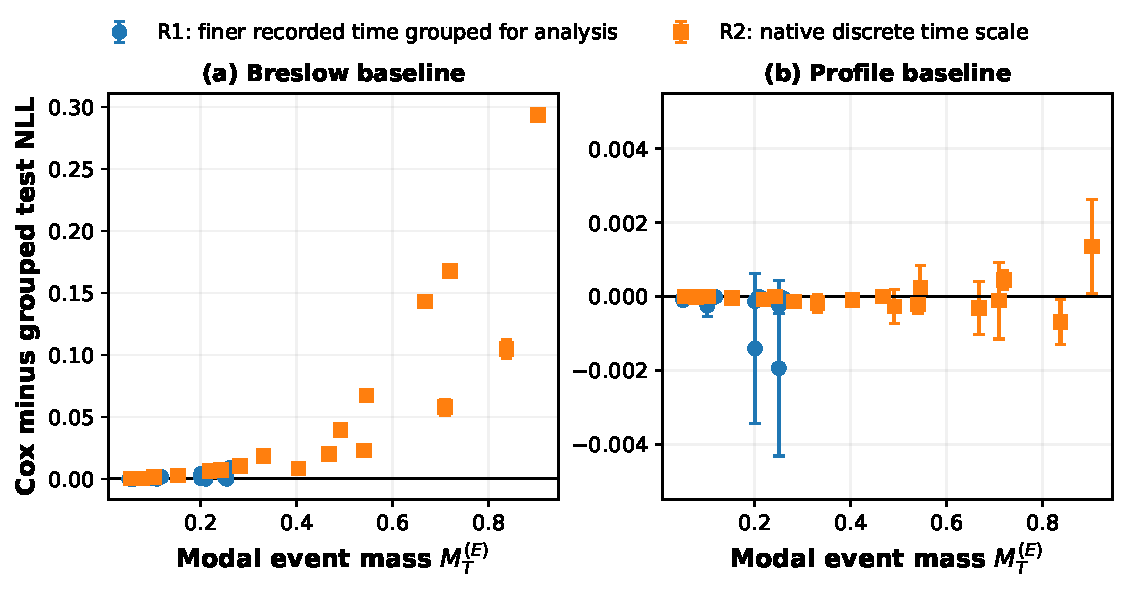
\includegraphics[width=\textwidth]{figures/F1_baseline_decomposition.pdf}
\caption{Baseline-estimator decomposition over all 34 main configurations. The two panels use the same Efron Cox coefficient and the same test observations. Panel (a) reconstructs the baseline with the Breslow estimator; panel (b) replaces only that baseline by the Kalbfleisch--Prentice/profile estimator. Error bars are Nadeau--Bengio corrected repeated-split standard errors. The vertical scales differ between panels so that the residual profile-baseline differences remain visible.}
\label{fig:baseline-decomposition}
\end{figure}
\FloatBarrier

\begin{table}[!htbp]
\caption{Representative baseline-decomposition results. The same Efron Cox coefficient is used in the Breslow and Kalbfleisch--Prentice columns. Positive differences favour the grouped joint maximum-likelihood fit. SE denotes the Nadeau--Bengio corrected repeated-split standard error.}
\label{tab:main-examples}
\centering
\small
\begin{tabular}{@{}lrrrrr@{}}
\toprule
Configuration & $M_T^{(E)}$ & $D_B$ & SE & $D_{KP}$ & SE \\
\midrule
support-pycox, $T=4$ & 0.261 & 0.00892 & 0.00173 & -0.00006 & 0.00007 \\
support2/slos, $T=6$ & 0.491 & 0.03928 & 0.00446 & -0.00027 & 0.00045 \\
drsa/clinic, $T=5$ & 0.837 & 0.10464 & 0.00762 & -0.00069 & 0.00060 \\
sparcs/drg302, $T=6$ & 0.903 & 0.29336 & 0.00261 & 0.00135 & 0.00128 \\
\bottomrule
\end{tabular}
\end{table}
\FloatBarrier

The largest standard-pipeline difference occurred for sparcs/drg302 at $T=6$: $D_B=0.29336$ with corrected SE 0.00261. With the coefficient and test rows unchanged, substitution of the profile baseline reduced the difference to $D_{KP}=0.00135$ with corrected SE 0.00128. Similar reductions occurred in clinic and support2. Among configurations with $|D_B|>10^{-4}$, the median descriptive baseline share was 100.9\%. Ratios above 100\% reflect small negative $D_{KP}$ values rather than an effect larger than the original difference.

The 20-split rerun also removed the sign-crossing pattern seen in the earlier, smaller experiment. For support2, $D_B$ decreased from 0.03928 at $T=6$ to 0.00041 at $T=60$ but remained positive. For the music cohort it decreased from 0.02025 at $T=6$ to 0.00028 at $T=60$ and again remained positive. We therefore do not estimate a universal or cohort-specific crossover threshold from these data.

These results do not imply that the Cox and grouped coefficient estimators are identical under ties. The large held-out likelihood differences produced by the usual Cox-Breslow prediction pipeline are therefore primarily associated with the baseline estimator. The comparison is especially clean because the two Cox columns use the same $\widehat\beta_E$.

\subsection{Independent SPARCS validation}
\label{sec:heldout}

To check whether the near-zero profile-baseline result was specific to the cohorts used to develop the comparison, four additional SPARCS APR-DRG groups were analysed. None was used in the preceding 34-configuration summary. Each group was capped at 50,000 observations and analysed at $T=6,15,30$ using 10 repeated splits.

\begin{table}[!htbp]
\caption{Independent SPARCS validation. Modal mass in this table is the modal mass of all recorded exits because that statistic was stored in the independent validation run. Positive differences favour the grouped joint fit.}
\label{tab:heldout}
\centering
\scriptsize
\begin{tabular}{@{}lrrrrrr@{}}
\toprule
Group & $T$ & Modal mass & $D_B$ & SE & $D_{KP}$ & SE \\
\midrule
drg640 & 6  & 0.9884 & 0.42344 & 0.00131 & 0.00340 & 0.00051 \\
drg640 & 15 & 0.6489 & 0.17770 & 0.00217 & 0.00048 & 0.00150 \\
drg640 & 30 & 0.5831 & 0.10006 & 0.00187 & 0.00067 & 0.00152 \\
drg560 & 6  & 0.9900 & 0.42706 & 0.00311 & 0.00188 & 0.00221 \\
drg560 & 15 & 0.6525 & 0.19123 & 0.00296 & 0.00017 & 0.00150 \\
drg560 & 30 & 0.6012 & 0.13561 & 0.00258 & 0.00040 & 0.00044 \\
drg540 & 6  & 0.9372 & 0.34261 & 0.00217 & 0.00455 & 0.00075 \\
drg540 & 15 & 0.7754 & 0.21119 & 0.00244 & 0.00175 & 0.00029 \\
drg540 & 30 & 0.4657 & 0.07957 & 0.00198 & 0.00017 & 0.00011 \\
drg720 & 6  & 0.4207 & 0.05641 & 0.00176 & 0.00037 & 0.00022 \\
drg720 & 15 & 0.1946 & 0.01167 & 0.00097 & -0.00001 & 0.00006 \\
drg720 & 30 & 0.0990 & 0.00306 & 0.00056 & -0.00001 & 0.00002 \\
\bottomrule
\end{tabular}
\end{table}
\FloatBarrier

All 12 $D_B$ values were resolved and positive. Three of the 12 $D_{KP}$ values were also resolved and positive: drg640 at $T=6$, and drg540 at $T=6$ and $T=15$. The profile-baseline residual therefore is not identically zero. It is small relative to the original effect: across the 12 rows it ranged from $-0.33\%$ to $1.33\%$ of $D_B$, corresponding to a baseline share between 98.7\% and 100.2\%. The residual was ordered by tie concentration in this validation set (Spearman correlation 0.853 with the stored modal-exit mass), but the sample is too small and the grid dependence too strong to justify a numerical threshold.

\subsection{Event concentration rather than censoring concentration}
\label{sec:event-sim}

On the native discrete cohorts, $M_T^{(A)}$ and $M_T^{(E)}$ move together, so their empirical correlations with $D_B$ do not identify which feature matters. A 27-cell simulation was therefore constructed to vary the concentration of censoring independently of the concentration of failures. Across these cells, the Spearman correlation between $D_B$ and the modal mass of all exits was $-0.1469$. The corresponding correlation with modal event mass was 0.8745. Events per interval had correlation 0.3777. These are average-rank Spearman coefficients. An earlier version of the analysis code assigned ordinal ranks to tied printed masses, giving $-0.1422$, 0.8742 and 0.3712 on the same 27 cells; the revision changes the statistic and not the simulation, and it does not alter the ordering of the three measures.

\begin{figure}[!htbp]
\centering
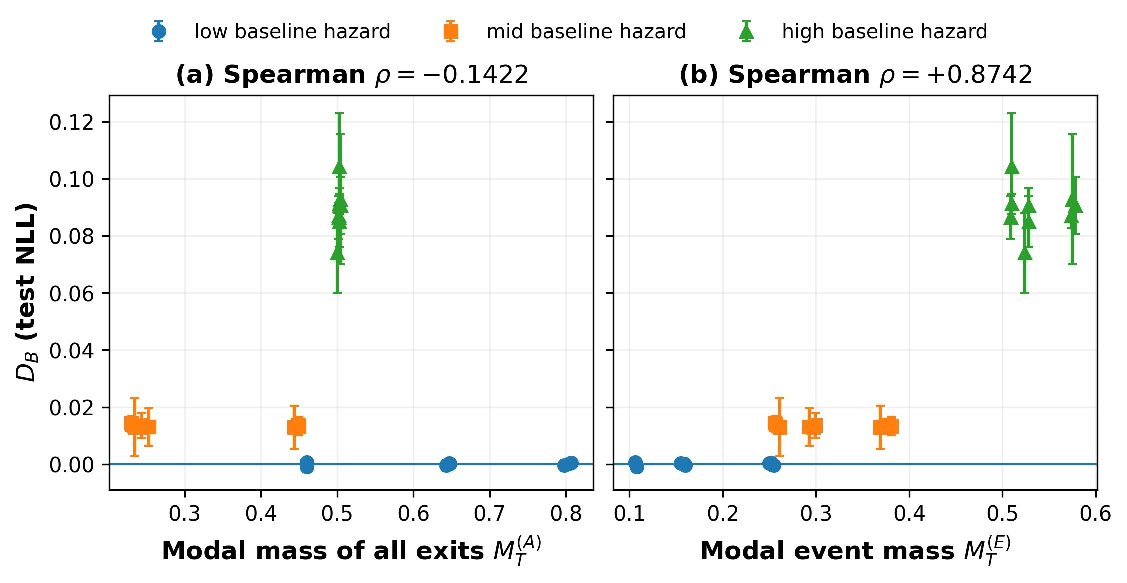
\includegraphics[width=\textwidth]{figures/F2_event_concentration.pdf}
\caption{Identified comparison of concentration measures in the 27-cell simulation. Baseline hazard level, sample size and grid size were crossed so that concentration of all exits could vary separately from concentration of failures. Modal mass of all exits does not order $D_B$ in this design (panel a), whereas modal event mass does (panel b). Error bars are corrected repeated-split standard errors.}
\label{fig:event-concentration}
\end{figure}
\FloatBarrier

Figure~\ref{fig:event-concentration} is consistent with the structure of tied risk-set approximations: simultaneous failures enter the tied event set, whereas a pile of administrative censoring observations in the last interval can make $M_T^{(A)}$ large without creating a tied failure set. We therefore use Eq.~\eqref{eq:modal-event} as the primary concentration diagnostic. It is an ordering variable, not a universal cutoff.

A second simulation checked a different possible interpretation. A continuous Weibull proportional hazards process was generated and then grouped exactly on the analysis grid. At $n=10{,}000$ without censoring and Weibull shape 0.8, the grouped coefficient bias stayed near 0.5\% for all tested grids. The Cox coefficient bias was 35.6\% at $T=2$, 20.5\% at $T=4$, 9.9\% at $T=8$, 3.0\% at $T=20$ and 1.2\% at $T=40$. The corresponding $D_B$ values were 0.17259, 0.10160, 0.04594, 0.01292 and 0.00341. Exactness of the grouped representation therefore does not imply equality of the two estimators after failure times have been tied. It guarantees correctness of the grouped complementary-log-log model under the simulated data-generating process.

\begin{figure}[!htbp]
\centering
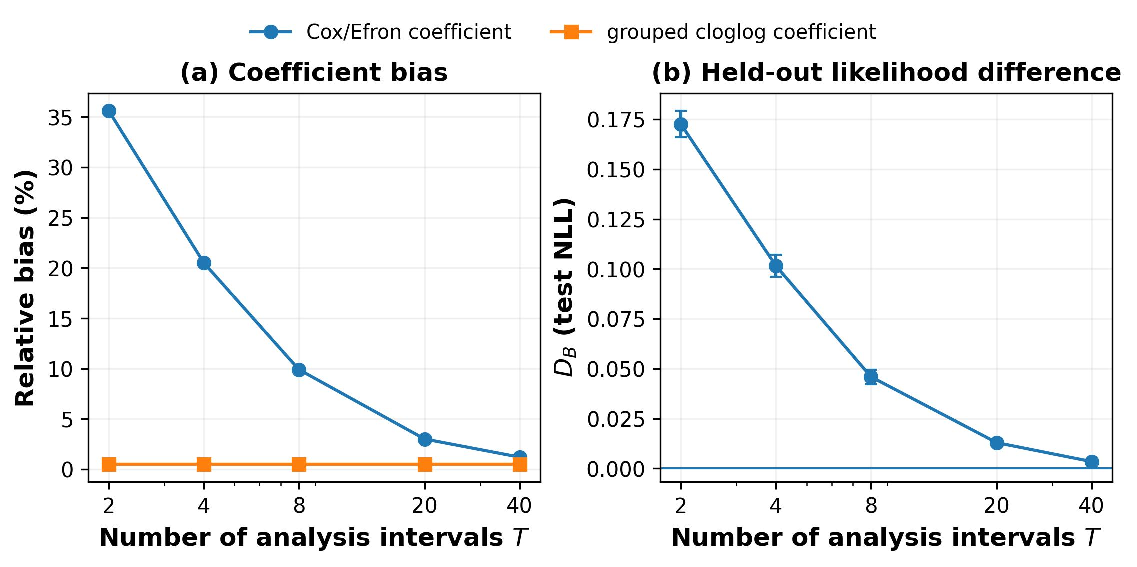
\includegraphics[width=\textwidth]{figures/F3_grouped_weibull.pdf}
\caption{Controlled Weibull proportional-hazards experiment with $n=10{,}000$, shape 0.8 and no censoring. Failure times were generated continuously and then grouped exactly on the analysis grid. The grouped complementary-log-log coefficient remains close to the generating value while the Cox/Efron coefficient is attenuated on coarse grids (panel a). The corresponding Cox-Breslow minus grouped test negative log-likelihood difference decreases as the grid is refined (panel b).}
\label{fig:weibull-grouping}
\end{figure}
\FloatBarrier

A further link-misspecification simulation generated discrete hazards from a logistic rather than complementary-log-log model. The correctly specified logit likelihood had the better link likelihood in all 16 tested cells, while the original grouped-versus-Cox $D_B$ remained positive in all 16. Thus $D_B$ should not be interpreted as a measure of whether the complementary-log-log link is correct.

\subsection{Censoring and grid sensitivity}
\label{sec:sensitivity}

The exact Bernoulli product in Eq.~\eqref{eq:grouped-likelihood} treats a subject censored in interval $t$ as exposed through the interval. This is exact only when censoring is aligned to the grid. In the four native-discrete cohorts used for the principal R2 comparison, the recorded censoring times were aligned in the tested configurations. A partial-interval likelihood changed $D_B$ only slightly: from $-0.00006$ to $-0.00019$ for support2 at $T=60$, from 0.06769 to 0.06717 for sparcs/drg302 at $T=30$, from 0.00923 to 0.00915 for clinic at $T=50$, and from 0.00047 to 0.00009 for music at $T=240$.

The R1 controls are different. The proportion of censored observations potentially off a grid boundary was 72.5\% for flchain, 32.0\% for support-pycox, 85.8\% for nwtco and 42.1\% for metabric in the audited configurations. The corresponding partial-interval sensitivity moved $D_B$ from 0.00002 to $-0.00401$, 0.00034 to $-0.00839$, $-0.00012$ to $-0.00271$, and $-0.00069$ to $-0.00873$. For this reason the R1 cohort results are not used as empirical proof that exact grouping forces the formulations to agree.

Grid construction also changes concentration. Equal-width, equal-count and native grids gave materially different modal masses in several cohorts. A concentration statistic must therefore be reported together with the grid convention. The experiments do not support a grid-independent tie threshold.

\section{Discussion}
\label{sec:discussion}

The theoretical and empirical results concern different parts of the same problem. The information calculation asks how much is lost when a continuous failure time is replaced by an interval label. The empirical decomposition asks why two procedures fitted to the same grouped observations can give different interval predictions. Conflating these questions leads to an overly simple interpretation of ties.

For the information question, Lemma~\ref{lem:exact} gives a finite-grid identity. The loss is strictly positive for every interval with positive integrated hazard. Under regular refinement, Theorem~\ref{thm:small-bin} recovers the classical quadratic grouping rate and gives its coefficient for the local proportional-hazards direction. Profiling an interval baseline preserves the quadratic rate, but the leading coefficient contains a subtraction for within-bin movement of the risk-set covariate mean. The result is useful mainly as a description of what grouping removes. It should not be read as a rule for choosing an artificial continuous resolution for data whose time scale is genuinely discrete.

For the prediction question, the large empirical difference was primarily a baseline-estimation effect. In the main 34 configurations, replacing the Breslow baseline by the Kalbfleisch--Prentice profile baseline while leaving the Efron coefficient unchanged reduced every resolved positive grouped advantage to an unresolved value. Independent validation did not give an exact null: three profile-baseline residuals were resolved. Their size was small, however, relative to the original Breslow differences. The data therefore support a narrower statement than a claim that grouped maximum likelihood and Cox regression are interchangeable. Under heavy ties, interval prediction from a Cox coefficient can depend materially on the baseline reconstruction; a profile-compatible baseline removes most of the observed likelihood gap.

This finding also clarifies the role of classical work on grouped failure times. Kalbfleisch and Prentice derived likelihood-based treatment of grouped Cox data and survivor estimation long before the present comparison \citep{kalbfleisch1973}. Allison described complementary-log-log event-history likelihoods in discrete time \citep{allison1982}, and Prentice and Kalbfleisch later considered mixed discrete and continuous Cox models \citep{prentice2003}. The contribution here is not a new baseline estimator. It is the decomposition of a modern prediction comparison under substantial ties, together with finite-grid information calculations and controlled tests of the concentration statistic.

The modal event mass proved more informative than the modal mass of all exits in the controlled simulation. This distinction is practical. Administrative censoring can dominate the final recorded category without creating simultaneous failures, whereas tied partial-likelihood approximations depend on the event set. Even modal event mass is only descriptive. Its value changes with grid construction, and the independent validation does not support a universal cutoff at which one method should replace another.

Several limitations remain. First, the empirical comparison uses a finite set of cohorts and grids. The four independent SPARCS groups strengthen the baseline decomposition but are drawn from the same administrative data system. Second, the profile-baseline calculation holds the Cox coefficient fixed; residual differences can therefore reflect the coefficient estimator, joint estimation of $\alpha$ and $\beta$, or finite-sample interaction between them. Third, full-interval grouped likelihood contributions require aligned censoring. The partial-interval sensitivity shows that this idealisation matters for some artificially binned continuous-time controls. Fourth, the profiled information theorem treats an interval-specific nuisance baseline on a refining grouped model and is not a full semiparametric efficient-information calculation for an unknown continuous baseline. Finally, the corrected repeated-split standard error accounts for overlap in repeated train--test splits but does not turn the collection of configurations into independent hypothesis tests \citep{nadeau2003}.

The practical implication is modest. When the inferential target is a Cox regression coefficient, the partial-likelihood analysis remains a natural choice. When the target is a full set of interval probabilities on a coarse scale, the baseline used after fitting the Cox coefficient deserves explicit attention. Under heavy event ties, the Kalbfleisch--Prentice/profile baseline provides a likelihood-compatible alternative to the usual Breslow reconstruction. Direct grouped maximum likelihood is another route to the same interval probability model, with the regression coefficient estimated jointly with the baseline.

\FloatBarrier
\section{Conclusion}
\label{sec:conclusion}

Coarse event times create both information loss and an estimation problem. These should be kept separate. Grouping a continuous proportional hazards process has an exact complementary-log-log representation, but observing only the interval still loses Fisher information. The finite-grid loss is strictly positive and has the usual quadratic small-bin order under regular refinement.

The empirical prediction gap has a different source. Across the main experiments, most of the advantage of grouped joint maximum likelihood over a standard Cox prediction pipeline disappeared when the same Cox coefficient was paired with the Kalbfleisch--Prentice profile baseline instead of the Breslow baseline. Small residual differences remained under the most concentrated ties in independent validation. Event-tie concentration, rather than concentration of censoring and failures together, was the more informative diagnostic.

These results argue against using the number of tied observations or a fixed crossover rule as a model-selection criterion. The observation scale, the event-tie structure, and the baseline estimator used to convert a fitted Cox coefficient into interval probabilities should be stated separately.

\section*{Statements and Declarations}

\subsection*{Funding}

The authors received no specific funding for this work.

\subsection*{Competing interests}

The authors declare that they have no financial or non-financial competing interests relevant to this work.

\subsection*{Author contributions}

Simhaa T. T. contributed to conceptualization, methodology, software, formal analysis, investigation, data curation, visualization, and preparation of the original manuscript. Sudheesh Kumar Kattumannil contributed to conceptualization, methodology, supervision, validation, and review and editing of the manuscript. Both authors reviewed and approved the submitted version and take responsibility for the work.

\subsection*{Ethics approval}

Not applicable. The study used publicly available, de-identified secondary datasets and involved no direct interaction with human participants.

\subsection*{Consent to participate}

Not applicable.

\subsection*{Consent for publication}

Not applicable.

\subsection*{Data availability}

All datasets analysed in this study are publicly available from their original sources. SUPPORT data are available through the Vanderbilt University Department of Biostatistics \citep{support1995,vanderbiltSupport2026}. SPARCS data are provided by the New York State Department of Health \citep{nysdoh2012sparcs}. The clinic and music datasets are distributed with the DRSA study \citep{ren2019drsa}. The remaining benchmark cohorts are documented in their original publications and public survival-analysis distributions \citep{kvamme2019pycox,curtis2012metabric,dispenzieri2012flchain,breslow1999nwtco,foekens2000rotterdam,schumacher1994gbsg,katzman2018deepsurv}. No new participant-level data were collected. Third-party participant-level datasets are not included in the code archive. Dataset-access instructions and frozen aggregate results are available at \url{https://doi.org/10.5281/zenodo.22347056}; users must obtain source data under the providers' applicable access conditions.

\subsection*{Code availability}

Code and frozen aggregate results are archived on Zenodo as version 1.0.0 at \url{https://doi.org/10.5281/zenodo.22347056} \citep{simhaa2026groupedcode}. Development source is available at \url{https://github.com/Simhaatt/grouped-ph-reproducibility}. The archive includes scripts for data preparation, model fitting, numerical verification, and regeneration of tables and figures from frozen outputs. Reproduction limitations are documented in the repository; third-party raw datasets are not redistributed.

\subsection*{Use of generative artificial intelligence}

Generative artificial intelligence tools, including Anthropic Claude and OpenAI ChatGPT, were used to assist with software implementation and debugging, planning and checking statistical analyses, interpretation of intermediate results, and drafting and revision of the manuscript. These tools were not used to generate, alter, or synthesize participant-level data. The authors reviewed the analysis code, numerical results, citations, and manuscript text, and take responsibility for the accuracy and integrity of the final work.

\bibliographystyle{spbasic}
\bibliography{references}

\end{document}
